\documentclass[tikz,border=10pt]{standalone}
\usepackage{tikz}
\usetikzlibrary{arrows.meta, positioning}

\newcommand{\til}{$\sim$}
\newcommand{\Dconst}{D\til 1}
\newcommand{\DSession}{D\til session.trend}
\newcommand{\Dsession}{D\til session}
\newcommand{\gconst}{$g_0$\til 1}
\newcommand{\gsession}{$g_0$\til session}
\newcommand{\gbehav}{$g_0$\til behaviour}
\newcommand{\gsessionbehav}{$g_0$\til session + behaviour}
\newcommand{\gmix}{$g_0$\til mixture}
\newcommand{\sigmaconst}{$\sigma$\til 1}
\newcommand{\sigmasession}{$\sigma$\til session}
\newcommand{\sigmamix}{$\sigma$\til mixture}

\begin{document}
% \begin{tikzpicture}[
%   model/.style={
%     draw, rounded corners,
%     align=center, font=\small,
%     minimum width=2.6cm, minimum height=0.9cm
%   },
%   modelH0/.style={
%     draw, rounded corners, fill=blue!8,
%     align=center, font=\small,
%     minimum width=2.6cm, minimum height=0.9cm
%   },
%   modelH1/.style={
%     draw, rounded corners, fill=red!8,
%     align=center, font=\small,
%     minimum width=2.6cm, minimum height=0.9cm
%   },
%   arrow/.style={-{Latex[length=2mm]}, thick, gray}
% ]

%% TREE 1 %%

\begin{tikzpicture}[
  model/.style={
    text=black,
    align=center, font=\small,
    minimum width=2.6cm, minimum height=0.9cm
  },
  modelH0/.style={
    text=blue,
    align=center, font=\small,
    minimum width=2.6cm, minimum height=0.9cm
  },
  modelH1/.style={
    text=red,
    align=center, font=\small,
    minimum width=2.6cm, minimum height=0.9cm
  },
  title/.style={
    text=black,
    align=center, font=\large,
    minimum width=2.6cm, minimum height=0.9cm
  },
  arrow/.style={-{Latex[length=2mm]}, thick, gray}
]


% ------------------------------------------------------------
% LEVEL 0: base model (no parameters)
% ------------------------------------------------------------
\node[modelH0] (base) at (0,0) {\Dconst, \gconst, \sigmaconst};

% ------------------------------------------------------------
% LEVEL 1: one added effect each
% ------------------------------------------------------------
\node[modelH1] (m11) at (-3.95,1.7) {\DSession, \gconst, \sigmaconst};
\node[modelH1] (m12) at (-3.95,1.2) {\Dsession, \gconst, \sigmaconst};
\node[modelH1] (m13) at (0.0,1.7) {\Dconst, \gsession, \sigmaconst};
\node[modelH0] (m14) at (0.0,1.2) {\Dconst, \gbehav, \sigmaconst};
\node[modelH1] (m15) at (3.95,1.7) {\Dconst, \gconst, \sigmasession};

% ------------------------------------------------------------
% LEVEL 2: two added effects (pairwise combinations)
% ------------------------------------------------------------
\node[model] (m21) at (-5.4,3.9) {\DSession, \gconst, \sigmasession};
\node[model] (m22) at (-5.4,3.4) {\Dsession, \gconst, \sigmasession};
\node[model] (m23) at (-5.4,2.9) {\DSession, \gsession, \sigmaconst};
\node[model] (m24) at (0.0,3.9) {\Dsession, \gsession, \sigmaconst};
\node[modelH1] (m25) at (0.0,3.4) {\DSession, \gbehav, \sigmaconst};
\node[modelH1] (m26) at (0.0,2.9) {\Dsession, \gbehav, \sigmaconst};
\node[modelH1] (m27) at (5.4,3.9) {\Dconst, \gsessionbehav, \sigmaconst};
\node[model] (m28) at (5.4,3.4) {\Dconst, \gsession, \sigmasession};
\node[modelH1] (m29) at (5.4,2.9) {\Dconst, \gbehav, \sigmasession};

% ------------------------------------------------------------
% LEVEL 3: three added effects
% ------------------------------------------------------------
\node[model] (m31) at (-6.4,6.1) {\DSession, \gbehav, \sigmasession};
\node[model] (m32) at (-6.4,5.6) {\Dsession, \gbehav, \sigmasession};
\node[model] (m33) at (-6.4,5.1) {\Dsession, \gsession, \sigmasession};
\node[model] (m34) at (0.0,6.1) {\DSession, \gsession, \sigmasession};
\node[model] (m35) at (0.0,5.6) {\Dconst, \gsessionbehav, \sigmasession};
\node[model] (m36) at (6.4,6.1) {\DSession, \gsessionbehav, \sigmaconst};
\node[model] (m37) at (6.4,5.6) {\Dsession, \gsessionbehav, \sigmaconst};

% ------------------------------------------------------------
% LEVEL 4: four added effects 
% ------------------------------------------------------------
\node[model] (m41) at (-6.4,7.3) {\DSession, \gsessionbehav, \sigmasession};
\node[model] (m42) at (6.4,7.3) {\Dsession, \gsessionbehav,
  \sigmasession};

% ------------------------------------------------------------
% Title :)
% ------------------------------------------------------------
\node[title] (t1) at (0.0, 8.1) {\underline{Tree 1}};

\end{tikzpicture}

%% TREE 2 %% 

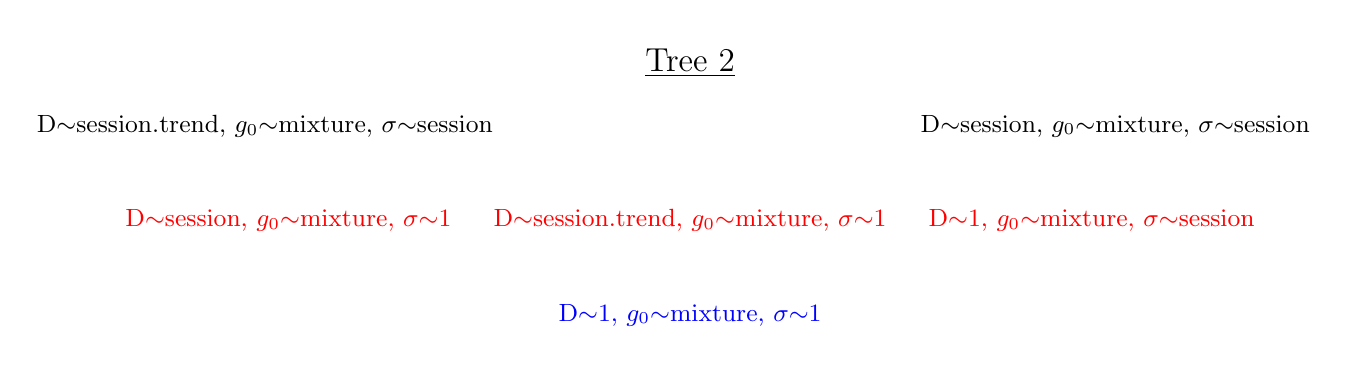
\begin{tikzpicture}[
  model/.style={
    text=black,
    align=center, font=\small,
    minimum width=2.6cm, minimum height=0.9cm
  },
  modelH0/.style={
    text=blue,
    align=center, font=\small,
    minimum width=2.6cm, minimum height=0.9cm
  },
  modelH1/.style={
    text=red,
    align=center, font=\small,
    minimum width=2.6cm, minimum height=0.9cm
  },
  title/.style={
    text=black,
    align=center, font=\large,
    minimum width=2.6cm, minimum height=0.9cm
  },
  arrow/.style={-{Latex[length=2mm]}, thick, gray}
]


% ------------------------------------------------------------
% LEVEL 0: base model (no parameters)
% ------------------------------------------------------------
\node[modelH0] (base) at (0,0) {\Dconst, \gmix, \sigmaconst};

% ------------------------------------------------------------
% LEVEL 1: one added effect each
% ------------------------------------------------------------
\node[modelH1] (m11) at (-5.1,1.2) {\Dsession, \gmix, \sigmaconst};
\node[modelH1] (m12) at (0.0,1.2) {\DSession, \gmix, \sigmaconst};
\node[modelH1] (m13) at (5.1,1.2) {\Dconst, \gmix, \sigmasession};

% ------------------------------------------------------------
% LEVEL 2: two added effects (pairwise combinations)
% ------------------------------------------------------------
\node[model] (m21) at (-5.4,2.4) {\DSession, \gmix, \sigmasession};
\node[model] (m22) at (5.4,2.4) {\Dsession, \gmix, \sigmasession};

% ------------------------------------------------------------
% Title :)
% ------------------------------------------------------------
\node[title] (t1) at (0.0, 3.2) {\underline{Tree 2}};

\end{tikzpicture}

%% TREE 3 %% 

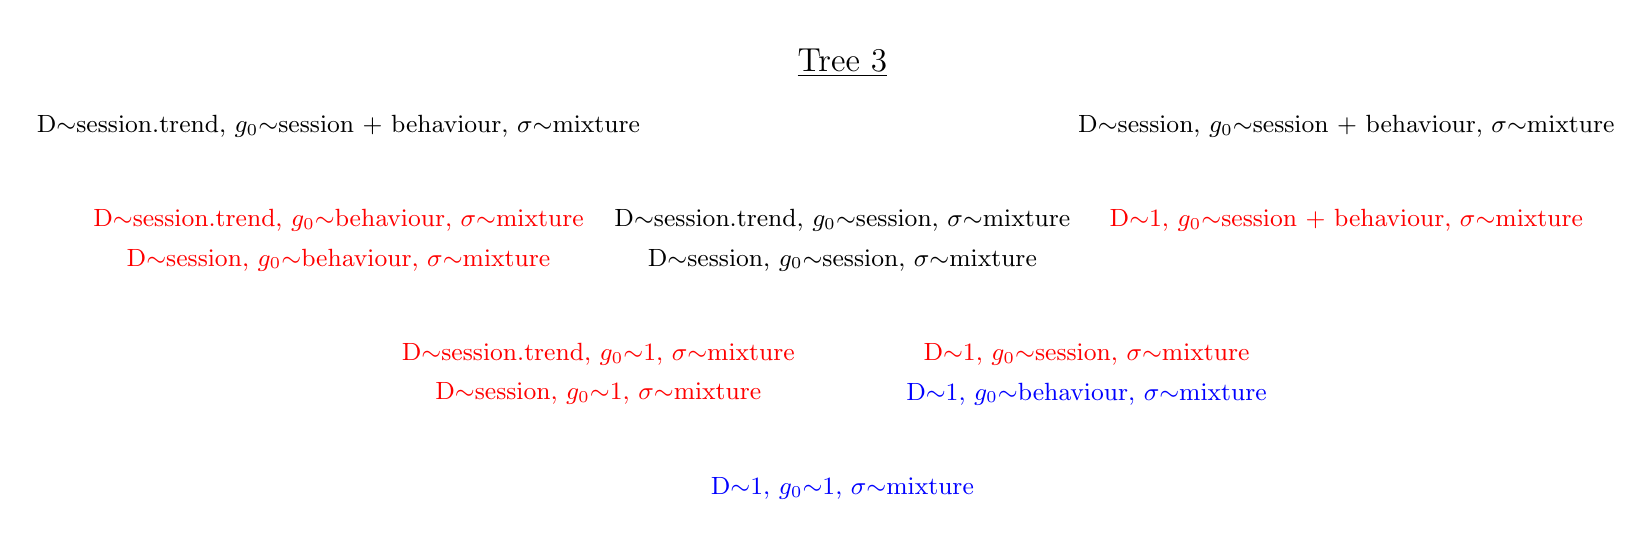
\begin{tikzpicture}[
  model/.style={
    text=black,
    align=center, font=\small,
    minimum width=2.6cm, minimum height=0.9cm
  },
  modelH0/.style={
    text=blue,
    align=center, font=\small,
    minimum width=2.6cm, minimum height=0.9cm
  },
  modelH1/.style={
    text=red,
    align=center, font=\small,
    minimum width=2.6cm, minimum height=0.9cm
  },
  title/.style={
    text=black,
    align=center, font=\large,
    minimum width=2.6cm, minimum height=0.9cm
  },
  arrow/.style={-{Latex[length=2mm]}, thick, gray}
]


% ------------------------------------------------------------
% LEVEL 0: base model (no parameters)
% ------------------------------------------------------------
\node[modelH0] (base) at (0,0) {\Dconst, \gconst, \sigmamix};

% ------------------------------------------------------------
% LEVEL 1: one added effect each
% ------------------------------------------------------------
\node[modelH1] (m11) at (-3.1,1.7) {\DSession, \gconst, \sigmamix};
\node[modelH1] (m12) at (-3.1,1.2) {\Dsession, \gconst, \sigmamix};
\node[modelH1] (m13) at (3.1,1.7) {\Dconst, \gsession, \sigmamix};
\node[modelH0] (m14) at (3.1,1.2) {\Dconst, \gbehav, \sigmamix};

% ------------------------------------------------------------
% LEVEL 2: two added effects (pairwise combinations)
% ------------------------------------------------------------
\node[modelH1] (m21) at (-6.4,3.4) {\DSession, \gbehav, \sigmamix};
\node[modelH1] (m22) at (-6.4,2.9) {\Dsession, \gbehav, \sigmamix};
\node[model] (m23) at (0.0,3.4) {\DSession, \gsession, \sigmamix};
\node[model] (m24) at (0.0,2.9) {\Dsession, \gsession, \sigmamix};
\node[modelH1] (m25) at (6.4,3.4) {\Dconst, \gsessionbehav, \sigmamix};

% ------------------------------------------------------------
% LEVEL 3: three added effects (pairwise combinations)
% ------------------------------------------------------------
\node[model] (m31) at (-6.4,4.6) {\DSession, \gsessionbehav, \sigmamix};
\node[model] (m32) at (6.4,4.6) {\Dsession, \gsessionbehav, \sigmamix};

% ------------------------------------------------------------
% Title :)
% ------------------------------------------------------------
\node[title] (t1) at (0.0, 5.4) {\underline{Tree 3}};

\end{tikzpicture}

%% TREE 4 %% 

\begin{tikzpicture}[
  model/.style={
    text=black,
    align=center, font=\small,
    minimum width=2.6cm, minimum height=0.9cm
  },
  modelH0/.style={
    text=blue,
    align=center, font=\small,
    minimum width=2.6cm, minimum height=0.9cm
  },
  modelH1/.style={
    text=red,
    align=center, font=\small,
    minimum width=2.6cm, minimum height=0.9cm
  },
  title/.style={
    text=black,
    align=center, font=\large,
    minimum width=2.6cm, minimum height=0.9cm
  },
  arrow/.style={-{Latex[length=2mm]}, thick, gray}
]


% ------------------------------------------------------------
% LEVEL 0: base model (no parameters)
% ------------------------------------------------------------
\node[modelH0] (base) at (0,0) {\Dconst, \gmix, \sigmamix};

% ------------------------------------------------------------
% LEVEL 1: one added effect each
% ------------------------------------------------------------
\node[modelH1] (m11) at (-5.1,1.2) {\DSession, \gmix, \sigmamix};
\node[modelH1] (m12) at (5.1,1.2) {\Dsession, \gmix, \sigmamix};
% ------------------------------------------------------------
% Title :)
% ------------------------------------------------------------
\node[title] (t1) at (0.0, 2.0) {\underline{Tree 4}};

\end{tikzpicture}


\end{document}